% Options for packages loaded elsewhere
\PassOptionsToPackage{unicode}{hyperref}
\PassOptionsToPackage{hyphens}{url}
%
\documentclass[
  12pt,
]{article}
\usepackage{lmodern}
\usepackage{amssymb,amsmath}
\usepackage{ifxetex,ifluatex}
\ifnum 0\ifxetex 1\fi\ifluatex 1\fi=0 % if pdftex
  \usepackage[T1]{fontenc}
  \usepackage[utf8]{inputenc}
  \usepackage{textcomp} % provide euro and other symbols
\else % if luatex or xetex
  \usepackage{unicode-math}
  \defaultfontfeatures{Scale=MatchLowercase}
  \defaultfontfeatures[\rmfamily]{Ligatures=TeX,Scale=1}
  \setmainfont[]{Times New Roman}
\fi
% Use upquote if available, for straight quotes in verbatim environments
\IfFileExists{upquote.sty}{\usepackage{upquote}}{}
\IfFileExists{microtype.sty}{% use microtype if available
  \usepackage[]{microtype}
  \UseMicrotypeSet[protrusion]{basicmath} % disable protrusion for tt fonts
}{}
\makeatletter
\@ifundefined{KOMAClassName}{% if non-KOMA class
  \IfFileExists{parskip.sty}{%
    \usepackage{parskip}
  }{% else
    \setlength{\parindent}{0pt}
    \setlength{\parskip}{6pt plus 2pt minus 1pt}}
}{% if KOMA class
  \KOMAoptions{parskip=half}}
\makeatother
\usepackage{xcolor}
\IfFileExists{xurl.sty}{\usepackage{xurl}}{} % add URL line breaks if available
\IfFileExists{bookmark.sty}{\usepackage{bookmark}}{\usepackage{hyperref}}
\hypersetup{
  pdftitle={State-Space Model to Estimate Salmon Escapement Using Multiple Data Sources},
  pdfauthor={Kevin E. See1,, Ryan N. Kinzer2, and Michael W. Ackerman1},
  pdfkeywords={escapement; Chinook; steelhead; salmon; Lower Granite Dam; state-space model; Bayesian model},
  hidelinks,
  pdfcreator={LaTeX via pandoc}}
\urlstyle{same} % disable monospaced font for URLs
\usepackage[margin=1in]{geometry}
\usepackage{longtable,booktabs}
% Correct order of tables after \paragraph or \subparagraph
\usepackage{etoolbox}
\makeatletter
\patchcmd\longtable{\par}{\if@noskipsec\mbox{}\fi\par}{}{}
\makeatother
% Allow footnotes in longtable head/foot
\IfFileExists{footnotehyper.sty}{\usepackage{footnotehyper}}{\usepackage{footnote}}
\makesavenoteenv{longtable}
\usepackage{graphicx,grffile}
\makeatletter
\def\maxwidth{\ifdim\Gin@nat@width>\linewidth\linewidth\else\Gin@nat@width\fi}
\def\maxheight{\ifdim\Gin@nat@height>\textheight\textheight\else\Gin@nat@height\fi}
\makeatother
% Scale images if necessary, so that they will not overflow the page
% margins by default, and it is still possible to overwrite the defaults
% using explicit options in \includegraphics[width, height, ...]{}
\setkeys{Gin}{width=\maxwidth,height=\maxheight,keepaspectratio}
% Set default figure placement to htbp
\makeatletter
\def\fps@figure{htbp}
\makeatother
\setlength{\emergencystretch}{3em} % prevent overfull lines
\providecommand{\tightlist}{%
  \setlength{\itemsep}{0pt}\setlength{\parskip}{0pt}}
\setcounter{secnumdepth}{-\maxdimen} % remove section numbering
% double spacing
\usepackage{setspace}
\doublespacing
% to double space figure captions
\usepackage{caption}
\captionsetup{font = doublespacing}

% line numbers
\usepackage{lineno}
\linenumbers
\usepackage{booktabs}
\usepackage{longtable}
\usepackage{array}
\usepackage{multirow}
\usepackage{wrapfig}
\usepackage{float}
\usepackage{colortbl}
\usepackage{pdflscape}
\usepackage{tabu}
\usepackage{threeparttable}
\usepackage{threeparttablex}
\usepackage[normalem]{ulem}
\usepackage{makecell}
\usepackage{xcolor}

\title{State-Space Model to Estimate Salmon Escapement Using Multiple Data Sources}
\author{Kevin E. See\textsuperscript{1,*}, Ryan N. Kinzer\textsuperscript{2}, and Michael W. Ackerman\textsuperscript{1}}
\date{May 10, 2021}

\begin{document}
\maketitle
\begin{abstract}
Accurate estimates of salmonids passing Lower Granite Dam on the Snake River, by species and origin, are a critical input to assessing the status and trends of various populations, as well as successful management of fisheries in the Snake River basin. Here we describe a state-space model that estimates such escapement past a dam by using window counts, passive integrated transponder (PIT) tag observations and data from an adult fish trap, accounting for issues such as nighttime passage, fallback and re-ascension, potential observation error at the window and uncertainty in the adult trap rate. We tested the approach using a simulation framework that mimicked several levels of observation error, differences between nighttime passage and re-ascension rates and the possibility of the adult trap being closed for some period of time. Our results demonstrate that the model produced unbiased estimates across all tested scenarios. We also applied this model to empirical data from the Lower Granite Dam to produce estimates of wild, clipped hatchery and unclipped hatchery spring/summer-run Chinook Salmon, \emph{Oncorhynchus tshawytscha}, and steelhead, \emph{O. mykiss}, from spawn years 2010-2019.
\end{abstract}

\textsuperscript{1} Biomark, Inc., 705 South 8th Street, Boise, Idaho, 83702, USA\\
\textsuperscript{2} Nez Perce Tribe, Department of Fisheries Resource Management, 14054 Burr Road, PO Box 1942, McCall, Idaho, 83638, USA

\textsuperscript{*} Correspondence: \href{mailto:Kevin.See@merck.com}{Kevin E. See \textless{}\href{mailto:Kevin.See@merck.com}{\nolinkurl{Kevin.See@merck.com}}\textgreater{}}

\hypertarget{introduction}{%
\section{Introduction}\label{introduction}}

Fish escapement refers to the number of adults that survive juvenile and subadult rearing, escape harvest, and achieve a size and age to potentially spawn (e.g., Bue et al. 1998). For anadromous fishes, escapement is often estimated at a fixed location in a river system prior to fish reaching their natal habitat to spawn (e.g., Woody 2004; Jasper et al. 2018). Escapement estimates facilitate effective fisheries management, particularly estimates of escapement for component groups (e.g., by stock, population, age, origin {[}wild, hatchery{]}, Hess et al. 2014; Steinhorst et al. 2017; Camacho et al. 2018) which provide valuable information that fisheries managers use to achieve sustainable harvest, while protecting small and vulnerable populations. Accurate escapement estimates are increasingly important for depleted populations as they inform status metrics (McElhany et al. 2000) and facilitate assessments of population viability, extinction risk (Northwest Fisheries Science Center 2015; Williams et al. 2016) and climate change vulnerability (Crozier et al. 2019).

Populations of Chinook Salmon \emph{Oncorhynchus tshawytscha} and anadromous steelhead trout \emph{O. mykiss} in the Snake River basin of Pacific Northwest, USA, are depleted following decades of substantial harvest and anthropogenic changes to their migration corridor (e.g., construction of hydroelectric projects on the Snake and Columbia rivers) and tributary habitats (Nehlsen et al. 1991; McClure et al. 2003; Northwest Fisheries Science Center 2015). As a result, most Snake River spring/summer-run Chinook Salmon (hereafter sp/sum Chinook Salmon) were classified as threatened in 1992 under the Endangered Species Act (ESA; Federal Registry Notice 57 FR 14653), and Snake River summer-run steelhead trout (hereafter steelhead) were listed as threatened five years later (Federal Registry Notice 62 FR 43937). Snake River sp/sum Chinook Salmon and steelhead have substantial cultural, recreational, commercial and subsistence value within the Snake River basin as well as in downstream corridors (i.e., Columbia River) and ocean fisheries. The aggregate escapement of Snake River sp/sum Chinook Salmon and steelhead populations, with the exception of Tucannon River (a tributary of the Snake River whose confluence is downstream of Lower Granite Dam {[}LGR{]}), is monitored at LGR located in southeast Washington; the final dam on the Snake River that returning adults must pass prior to heading to tributary spawning locations. Many fisheries management and conservation actions are made based on estimates of escapement by species and origin at LGR (NPCC 2014; Northwest Fisheries Science Center 2015; National Marine Fisheries Service 2019). As an example, tribal ceremonial and subsistence harvest rates in the region are informed by escapement at LGR; additionally, the openings, closures and bag limits of fisheries targeting hatchery fish, both upstream in Snake River fisheries and downstream in mainstem Snake and Columbia rivers, are informed by escapements at LGR (U.S. v Oregon 2018).

The majority of sp/sum Chinook Salmon and steelhead returning to the Snake River must ascend a fish ladder on LGR before migrating upriver. Fish management agencies previously used counts of fish, by species, passing an observation window within the fish ladder as a census of fish escaping past the dam. For both species, total escapement was then parsed into groups (e.g., wild, hatchery) using observed marks and genetic data from a sample of fish captured at an adult trap located on the fish ladder upstream of the observation window (Steinhorst et al. 2017; Camacho et al. 2018; Steele et al. 2019). Treating window counts as a census proved beneficial as being an easy, straight-forward method ascertained in near real-time. Moreover, downriver fisheries management arenas have used window counts at lower-river dams as escapement estimates for the past several years, and consistency in methods is often desirable for management decision making (Joint Columbia River Management Staff 2019).

However, using window counts as a census of fish passing LGR can be problematic as it fails to account for multiple sources of uncertainty and disregards known biological processes. Typically, the observational error rates of sp/sum Chinook Salmon and steelhead counted passing a window on the fish ladder, using both in-person and video methods, are unknown, and sampling error rates are ignored. Hatch et al. (1994) conducted a study of the counting system at LGR, and found that sp/sum Chinook Salmon were undercounted at the window by in-person window counters when compared to video counts. There was also a significant difference between daily standard counts (16 or 10 hours per day) and daily 24-hour video counts; the undercounting was attributed to a significant nighttime passage rate (crossing while the counting window was closed) with an estimated 3.5\% of sp/sum Chinook Salmon and 6.6\% of steelhead adults passing during ``nighttime'' hours. They also found some species misidentification issues, which could result in either under- or over-counting of a particular species. While that study identified potential issues with the current window counting procedure, it was only conducted in a single year, nearly 30 years ago, and at a time when sp/sum Chinook Salmon and steelhead total returns were typically lower than in the past decade.

One additional biological process, the fallback and re-ascension of adult migrants at the dam, should also be accounted for to estimate the true escapement of these species at LGR. Adult fish that migrate through the ladder and past the dam may fallback over the dam (e.g., over a spillway, through navigation locks) and later may re-ascend the fish ladder again (Boggs et al. 2004) and be counted multiple times at the window (re-ascension). Whereas unaccounted nighttime passage can lead to an underestimate in escapement, both fallback without and with re-ascension instead potentially lead to an overestimate of escapement (Dauble and Mueller 2000). Previously, it has often been assumed that these two biological processes essentially cancel each other out, resulting in window counts that provide an unbiased estimate of escapement (Camacho et al. 2018), which may be true in many or most years, but perhaps not always.

In this study, we describe a novel method to estimate aggregate and group escapements which incorporate all sources of known uncertainty and demonstrate that the estimation method is essentially unbiased, thus better informing conservation and management decision making. We also test whether observed nighttime passage and fallback/re-ascension rates are typically equal. Our method for estimating species-specific escapement past LGR incorporates window counts, data from the adult fish trap located on the ladder, and passive detections of adults in the ladder from fish previously tagged with passive integrated transponder (PIT) tags to explicitly model nighttime passage, re-ascension, and observation error using a state-space approach (Royle and Dorazio 2008) which separates process variance (e.g., week to week variance in true escapement) from observational variance (e.g., observation error at the window, or sampling variance at the trap). To meet desired management and conservation objectives, modeled escapement includes estimates of uncertainty and is parsed into weekly strata. Further, total and weekly estimates are divided into three origin groups: wild fish, hatchery fish with a clipped adipose fin, and unclipped hatchery fish. Our model is implemented in the \textbf{ST}ate-space \textbf{A}dult \textbf{D}am \textbf{E}scapement \textbf{M}odel (STADEM) package for the statistical software R (R Core Team 2020), and is available for download or installation from \url{https://github.com/KevinSee/STADEM}. To validate the STADEM results, we simulated 12 scenarios with varying trapping rates, fallback and re-ascension rates, nighttime passage rates, and window count error rates and compared STADEM results to the simulated ``truth''. Then, as a case study, we applied this model to sp/sum Chinook Salmon and steelhead returns at LGR for spawn years 2010 - 2019.

\hypertarget{methods}{%
\section{Methods}\label{methods}}

\hypertarget{data-requirements}{%
\subsection{Data Requirements}\label{data-requirements}}

Data sources for STADEM included 1) counts of fish migrating past the observation window located on the adult fish ladder at LGR, 2) information from adults captured at a fish trap located in the fish ladder, and 3) observations of fish PIT tagged prior to arriving at LGR and detected at arrays in the adult fish ladder. Below, we describe each of the data sources in more detail as they pertain to LGR; similar data could likely be obtained from other species passing LGR (e.g., fall Chinook Salmon) or other fish passage facilities (e.g., Bonneville Dam).

\hypertarget{window-counts}{%
\subsubsection{Window Counts}\label{window-counts}}

Daily counts of adult sp/sum Chinook Salmon and steelhead passing the observation window located on the LGR fish ladder were compiled and provided by the US Army Corps of Engineers. When summed, they provide an estimate of the number of fish ascending and passing LGR each season. Window counts were made for each species using direct in-person visual monitoring and video monitoring during daytime hours (Hatch et al. 1994). Direct visual monitoring occurred during peak run times (April 1 -- October 31) for 16 hours per day (0400 -- 2000 hours). Video monitoring occurred during the beginning and tail ends of the adult runs (March 1 -- March 31 and November 1 -- December 31) for 10 hours per day (0600 -- 1600 hours) (USACE 2015). During direct visual monitoring, observers recorded each adult (≥ 30cm), by species, passing the window for 50 minutes of each hour of operation. The sum of the daily 50-minute counts were then multiplied by 1.2 to account for the 10 minutes each hour when fish were not counted. Daytime window counts were not expanded for fish that may have ascended the ladder outside of operational hours (i.e., nighttime passage) (USACE 2015). Window counts were accessed through the Columbia Basin Research Data Access in Real Time (DART) website, \url{www.cbr.washington.edu/dart/query/adult_daily}, using their window count query. Counts were provided for each day the fish ladder was open to passage, and had already been expanded by 1.2.

\hypertarget{adult-fish-trap-data}{%
\subsubsection{Adult Fish Trap Data}\label{adult-fish-trap-data}}

The second source of data are from a sample of fish collected in the adult trap as they migrated past LGR (Ogden 2016a). The trap, also located within the adult fish ladder and upstream of the observation window, provides an opportunity to collect biological data (e.g., phenotypic origin {[}wild, hatchery{]}, tissue sample for genetic data, length, scale sample for age, sex) from captured adults which allows for decomposition of the escapement into specific groups (e.g., Camacho et al. 2018; Steinhorst et al. 2017). The trap was operational for 24 hours per day and randomly sampled the run by opening four times per hour for a length of time determined by a set daily trapping rate. The trap rate was determined by a committee of collaborating management agencies with a goal of capturing a target number of wild fish while also balancing fish handling concerns. Trap sample rates were typically 10-25\%, but fluctuated throughout the season due to, for example, high water temperatures, decreased flows, trap malfunctions and/or closures, fish handling logistics, in-season forecast adjustments, or adjustments due to shifting species composition throughout the year.

All captured fish were anesthetized, identified to species, examined for existing marks or tags, measured for fork length, and visually identified as wild or hatchery. The most widely used marking of hatchery fish is a clipped (removed) adipose fin, although coded wire tags are also used in less than 10\% of the hatchery releases. Some subset of hatchery fish are either intentionally or unintentionally released without a clipped adipose fin, and these are referred to as unclipped hatchery fish, or hatchery no-clips. For adults with intact adipose fins (unclipped), which includes wild and hatchery no-clip individuals, either a portion or all of the fish trapped (depending on the year) had scale and genetic tissue samples taken. Scale samples were used to estimate age (Wright et al. 2015) and genetic tissue samples were used to determine sex (Campbell et al. 2012) and estimate the location of origin of wild fish using genetic stock identification (e.g., Hargrove et al. 2019). Prior to 2013, only fish determined to be wild in origin at the trap were sampled for scale and genetics. Starting in 2013, every unclipped sp/sum Chinook Salmon and steelhead trapped at LGR was genotyped to simplify collaborative logistics and to better estimate the true proportion of unclipped hatchery fish that can otherwise appear phenotypically wild. Camacho et al. (2018) provide further details on trap sample rates and valid sample selection. Prior to release, all non-PIT tagged fish with an intact adipose fin (i.e., putatively wild) received a PIT tag. Final determination of wild, clipped hatchery, or unclipped hatchery origins were assigned using a post-hoc analysis of marks and tags, including parentage-based tagging based on the genetic samples taken (Steele et al. 2013, 2019). Data from the adult trap were collected and managed by multiple agencies and were made available by the Idaho Department of Fish and Game (Camacho et al. 2018).

\hypertarget{pit-tag-data}{%
\subsubsection{PIT Tag Data}\label{pit-tag-data}}

The last source of data were observations of PIT tagged adult sp/sum Chinook Salmon and steelhead at PIT tag detection sites located in the LGR fish ladder. These observations provide data related to 1) an estimate of the ``true'' trap rate for the adult fish trap, 2) a nighttime passage rate, and 3) a re-ascension rate. Detections used in the model included all fish that were previously PIT tagged as juveniles or adults prior to arriving at LGR (i.e., does not include newly tagged adults at the dam) and detected at adult detection sites in the dam passage system. PIT tag data were provided through DART and the adult ladder PIT tag query; \url{http://www.cbr.washington.edu/dart/query/pitadult_obsyr_detail}.

\hypertarget{model-framework}{%
\subsection{Model Framework}\label{model-framework}}

\hypertarget{total-and-weekly-escapement}{%
\subsubsection{Total and Weekly Escapement}\label{total-and-weekly-escapement}}

Escapement at LGR is estimated by combining two independent observations, trap catches and window counts, of the true number of fish crossing the dam in a state-space model (Royle and Dorazio 2008), with a weekly time-step. Both are assumed to be corrupted observations of the true unknown number of fish crossing LGR each week. We chose to use a weekly time-step to ensure sufficient sample sizes of PIT tag detections within each time strata, but this choice could be easily modified. The log of the true number of fish crossing during time-step \(t\), (\(X_t\)), is modeled as a random walk process (Shumway and Stoffer 2010), with \(e_t\) representing the process errors drawn from a normal distribution with variance \(\sigma^2_X\).

\begin{equation}
  \begin{aligned}
    \ln \left( X_{t} \right) &= \ln \left( X_{t-1} \right) + e_t \\
    e_t &\sim \text{Normal}(0, \sigma^2_X)
  \end{aligned}
\end{equation}

The number of fish caught in the trap, \(Y^T_t\), for week \(t\) is modeled as a binomial process based on the unknown true trap rate that week, \(\nu_t\), and the unknown true number of fish crossing the dam that week, \(X_t\).

\begin{equation}
  Y^T_t \sim \text{Bin} \left( \nu_t, X_t \right)
\end{equation}

The set trapping rate (i.e., the pre-determined time that the trap is open each hour to trap adults) does not always reflect the true trapping rate or proportion of fish actually captured in the trap due to various issues including trap malfunctions, separation-by-code fish opening the trap more frequently than expected, and process error (pulses or lack thereof of passing adults), among others. Therefore, we use a mark-recapture approach to estimate a ``true'' trapping rate, \(\nu_t\). The estimate of the true weekly trap rate is derived based on previously PIT-tagged sp/sum Chinook Salmon and steelhead that are crossing LGR that week, and uses a Lincoln-Peterson mark-recapture model (Seber 2002).

\begin{equation}
  m_t \sim \text{Bin} \left( \nu_t, M_t \right)
\end{equation}

The fish, from both species, caught in the trap that week are considered the ``mark'' group (\(m_t\)), and all the previously PIT tagged fish who are detected at the upper end of the LGR fish ladder that week are considered the second ``capture'' group, \(M_t\) (which includes recaptures of the ``marked'' fish). The proportion of previously marked fish that are caught in the adult trap, \(m/M\) can be modeled with a binomial distribution using the same trap rate parameter, \(\nu_t\). Although the group of previously PIT tagged fish is not assumed to be representative of the overall run, the rate at which they are caught in the trap should be the same rate that the overall run experiences. The more tagged fish crossing the dam in a particular week, the more certain we can be of the true trap rate.

The number of fish counted at the window, \(Y^W_t\), is modeled as a (potentially) over-dispersed negative binomial process, with an expected value of \(X_t^{day}\), the number of fish crossing the dam while the window is open. This is simply the total number of fish crossing that week, \(X_t\), multiplied by the proportion of fish crossing while the window is open for counting, \(\theta_t\). In the formula below, \(p_t\) is the probability parameter and \(r\) is the size parameter of a negative binomial distribution (as defined in Plummer (2019)). If \(r\) is estimated to be small it provides evidence for over-dispersion, and as it grows very large, the negative binomial distribution behaves like a Poisson distribution.

\begin{equation}
  \begin{aligned}
    X_t^{day} &= X_t * \theta_t \\
    p_t &= \frac{r}{\left( r + X_t^{day} \right)} \\  
    Y^W_t &\sim \text{NegBin} \left( p_t, r \right) \\
  \end{aligned}
\end{equation}

Thus, the unknown true number of fish crossing LGR each week, \(X_t\), is estimated from two different data sources: window counts and fish sampled in the trap. The window counts provide an estimate (with some potential observer error) of the fish crossing during daytime hours, while the fish in the trap, when expanded by the estimated true trap rate, provide an estimate of the total fish crossing that week. The use of both estimates allows for an estimation of observer error in the window counts which has previously been inestimable. For weeks when the trap is down, STADEM relies exclusively on the window counts and nighttime passage data, but there will be more uncertainty in the estimates.

\hypertarget{daytime-passage-and-re-ascension-rates}{%
\subsubsection{Daytime Passage and Re-ascension Rates}\label{daytime-passage-and-re-ascension-rates}}

There are two processes that must be accounted for to correct any bias in the window counts: first, the proportion of fish that cross the dam while the window is closed for counting (nighttime passage rate), and second, the proportion of fish that cross the dam multiple times (re-ascension rate) and therefore potentially counted multiple times. Both rates can be estimated from previously PIT tagged fish that are crossing the dam each week.

The nighttime passage rate is just the complement of the rate of fish passing during the day when the window is operating. The daytime passage rate for week \(t\), \(\theta_t\), is modeled as a random walk process (with deviations, \(g_t\), drawn from a normal distribution with variance \(\sigma^2_{\theta}\)) and estimated from a binomial distribution based on the number of PIT tags observed to cross the dam during operational hours, \(y^{day}_t\), and the total number of PIT tags observed to cross the dam at any point that week, \(N_t\) (Shumway and Stoffer 2010).

\begin{equation}
  \begin{aligned}
    y^{day}_t &\sim \text{Bin} \left(\theta_t, N_t \right) \\
    \text{logit} (\theta_{t}) &= \text{logit} \left( \theta_{t-1} \right) + g_t \\
    g_t &\sim \text{Normal}(0, \sigma^2_\theta) \\
  \end{aligned}
\end{equation}

The number of total fish crossing LGR differs from the number of unique fish crossing LGR because some fish fallback and re-ascend the dam. These fish are potentially double-counted (or more) at the window, and have the potential to be caught in the fish trap more than once. The number of tags known to be re-ascending the dam each week, \(y^{reasc}_t\), is modeled as a binomial process based on the estimated re-ascension rate, \(\eta_t\), and the total number of tags crossing the dam that week, \(N_t\). The logit of the re-ascension rate is modeled as a random walk process similar to daytime passage (Shumway and Stoffer 2010), with deviations, \(f_t\), drawn from a normal distribution with variance \(\sigma^2_\eta\).

\begin{equation}
  \begin{aligned}
    y^{reasc}_t &\sim \text{Bin} \left(\eta_t, N_t \right) \\
    \text{logit} \left( \eta_{t} \right) &= \text{logit} \left(\eta_{t-1} \right) + f_t \\
    f_t &\sim \text{Normal}(0, \sigma^2_\eta)
  \end{aligned}
\end{equation}

We looked for differences in weekly nighttime passage and re-ascension rates estimated using wild fish only, versus combining hatchery and wild fish together, and found no difference. Additionally, sample sizes of observed tags during most weeks are small, and may prohibit reliable estimation of rates for individual wild or hatchery stocks. Therefore, we combine wild and hatchery PIT tagged fish observations to estimate common nighttime passage and re-ascension rates to increase sample sizes.

\hypertarget{origin-proportions}{%
\subsubsection{Origin Proportions}\label{origin-proportions}}

After estimating the total number of fish to have crossed LGR each week, \(X_t\), the total must be further refined into the number of wild fish, \(X_{w,t}\), hatchery clipped fish, \(X_{hc,t}\) and hatchery no-clip fish, \(X_{hnc, t}\). This is done by estimating a weekly origin proportion vector, \(\omega_t\) based on the random sample of fish caught in trap that week, \(Y^T_t\). The observed number of wild, \(Y^T_{w,t}\), hatchery clipped, \(Y^T_{hc,t}\), and hatchery no-clip, \(Y^T_{hnc,t}\), fish caught in the trap that week is assumed to come from a multinomial distribution with probability vector \(\omega_t\). The log-odds ratio of the proportions in \(\omega_t\), in relation to the proportion of clipped hatchery fish \(\omega_{hc,t}\) (\(\phi_{w,t}\) and \(\phi_{hnc,t}\)), is modeled as a random walk, so it can change through time, while smoothing over large weekly fluctuations in the proportions due to small sample size. This allows the proportions of wild, hatchery clipped and hatchery no-clip fish to shift throughout the season, based on the data available from the fish trap. The random walk deviations, \(d_{w,t}\) and \(d_{hnc,t}\), are drawn from the same normal distribution with variance \(\sigma^2_\omega\).

\begin{equation}
  \begin{aligned}
    \left( Y^T_{w,t}, Y^T_{hc,t}, Y^T_{hnc,t} \right) &\sim \text{Multinom} \left( \omega_t, Y^T_t \right) \\
    \omega_t &= \frac{\exp(\phi_t)}{\sum{\exp(\phi_t})} \\
    \phi_{hc,t} &= 0 \\
    \phi_{w,t} &= \ln \left( \frac{\omega_{w,t}}{\omega_{hc,t}} \right) \\
    \phi_{hnc,t} &= \ln \left( \frac{\omega_{hnc,t}}{\omega_{hc,t}} \right) \\
    \phi_{w,t} &= \phi_{w, t-1} + d_{w,t} \\
    \phi_{hnc,t} &= \phi_{hnc, t-1} + d_{hnc,t} \\
    d_{w,t} &\sim \text{Normal}(0, \sigma^2_\omega) \\
    d_{hnc,t} &\sim \text{Normal}(0, \sigma^2_\omega) \\
  \end{aligned}
\end{equation}

Finally, the number of unique fish by origin crossing LGR each week (\(X_{w,t}\), \(X_{hc,t}\), and \(X_{hnc,t}\)) is the product of the total fish crossing that week, \(X_t\), multiplied by one minus the re-ascension rate, \((1 - \eta_t)\), and the origin proportion vector, \(\omega_t\).

\begin{equation}
  \begin{aligned}
    \begin{bmatrix} X_{w,t} \\ X_{hc,t} \\ X_{hnc,t} \end{bmatrix}
    &= X_t * (1 - \eta_t) * \begin{bmatrix} \omega_{w,t} \\ \omega_{hc,t} \\ \omega_{hnc,t} \end{bmatrix}
  \end{aligned}
\end{equation}

In practice, the total number of fish crossing LGR each week, \(X_t\), could be split into other discrete groups if desired; for example, individual wild stocks using genetic stock identification or hatchery stocks with parentage based tagging (Steele et al. 2019). A graphical depiction (directed acyclic graph) of the model framework described above is found in Figure \ref{fig:dag-fig}.

\hypertarget{model-fitting}{%
\subsubsection{Model Fitting}\label{model-fitting}}

The model was fit using the JAGS program (Plummer 2019), run with R software (R Core Team 2020). The STADEM package is available from the primary author at \url{https://github.com/KevinSee/STADEM}, and requires the use of the JAGS software (Plummer 2019) for Bayesian inference. Variance parameters \(\sigma_X, \sigma_\eta, \sigma_\theta\), and \(\sigma_\omega\), as well as the initial abundance, \(X_1\), and the overdispersion parameter of the negative binomial, \(r\), were given half-Cauchy priors with mean of 0 and scale of 100. The initial daytime passage and re-ascension rates, \(\theta_1\) and \(\eta_1\) were given Uniform(0,1) priors. Finally, \(\phi_{w,1}\) and \(\phi_{hnc,1}\) were given priors of Uniform(-3,3), in an effort to make \(\omega_1\) as uninformative as possible.

\hypertarget{simulations}{%
\subsection{Simulations}\label{simulations}}

We tested the STADEM model on a variety of simulated data sets, constructed to mimic some dynamics of interest at LGR. These simulated data sets each contained a fixed number of unique adult fish of known origin crossing a dam, from a total of 25 fictional populations with differential run-timing (i.e., date of passage at LGR). Each simulated fish was given a date of ladder ascension, based on its population and the range of observed run timing for that population. Each fish was also simulated to cross the dam either while the window was open for counting, or not, and was given the chance to be ``caught'' in the simulated fish trap given the week when it ascended the dam, and the known trap rate that week. Fallback and re-ascension behavior was also simulated, with each fish having the possibility of falling back and re-ascending the ladder up to three times.

Our objective was to assess STADEM model estimates of origin-specific (wild, hatchery, hatchery no-clip) escapement for accuracy and precision, given a known simulated ``truth'', under different possible conditions. We developed those conditions from the combinations of two trap rate scenarios (constant and shut down for 3 weeks), two fallback/re-ascension and nighttime passage combinations (equal and unequal), and three window count error rates (none, low and high); resulting in twelve different scenarios overall (Table \ref{tab:lgr-sim-tab}). The simulation parameters such as proportion of origin, run-timing, nighttime passage rates, fallback and re-ascension rates and trap rates were based on observed values at LGR between 2010-2015. We generated 500 simulations for each scenario, and ran STADEM on each one, resulting in a total of 6,000 model runs. Further details about the simulation procedures can be found in \protect\hyperlink{append1}{Appendix A}.

To assess the performance of the model, we evaluated the estimates of origin-specific escapement by several measures. Accuracy was captured by the mean relative bias: the difference between the simulated ``truth'' and the STADEM estimate for each simulation, divided by the simulated ``truth''. We estimated the precision by examining the average coefficient of variation (CV) of the estimates. We calculated the root mean squared error (RMSE) as the square root of the mean of the squared bias in the estimate, which is equivalent to the square root of the variance of the estimator plus the square of the expected bias. Finally, we evaluated whether estimates of uncertainty were appropriate by calculating coverage probabilities to determine what proportion of the model results generated an estimated 95\% credible interval that contained the simulated true value. To compare the STADEM results directly to window counts, we compared the model estimates of total unique fish and the simulated window counts to the simulated number of unique fish.

\hypertarget{lower-granite-dam-application}{%
\subsection{Lower Granite Dam Application}\label{lower-granite-dam-application}}

We applied STADEM to empirical data from LGR for sp/sum Chinook Salmon and steelhead returning to the Snake River during spawn years 2010 to 2019. Window counts for both species were accessed from DART via functions within STADEM. For sp/sum Chinook Salmon, a spawn year refers to adults that migrate past the dam prior to August 17 each year and spawn that late summer and fall. For steelhead, the spawn year is defined as steelhead that migrate past LGR starting July 1 the previous year and prior to June 30 of the given year (e.g., spawn year 2017 steelhead migrate past LGR between July 1, 2016 and June 30, 2017). Data from the adult trap were made available by Idaho Department of Fish and Game, and adult PIT tag detection data within the fish passage ladder at LGR were accessed through DART and the adult ladder PIT tag query (\url{http://www.cbr.washington.edu/dart/query/pitadult_obsyr_detail}).

All data used in this manuscript, as well as associated code for both the simulations and the LGR application, can be found at \href{\%5Bhttps://www.github.com/KevinSee/ManuscriptSTADEM\%5D}{https://www.github.com/KevinSee/ManuscriptSTADEM}.

\hypertarget{results}{%
\section{Results}\label{results}}

\hypertarget{simulations-1}{%
\subsection{Simulations}\label{simulations-1}}

The evaluation statistics (relative bias, CV, RMSE, coverage probabilities) to assess performance of the STADEM model were very similar among hatchery clipped (N = 70,000), hatchery no-clip (N = 5,000) and wild fish (N = 25,000). In the interest of brevity, we only present the results from wild fish here, which corresponds to a moderate sized escapement relative to the hatchery clipped and hatchery no-clip groups.

STADEM results showed similar patterns for estimates of unique total fish and unique wild fish, in that both were unbiased with similar variance in the estimator across all scenarios as seen in the consistent interquartile range in the boxplots of Figure \ref{fig:rel-bias-lgd}. For unique total fish, window counts were unbiased, except in scenarios when night passage and re-ascension rates were not equal (N-R). In those scenarios, they were biased by nearly 5\% (Figure \ref{fig:rel-bias-lgd}), the designed simulated difference between night passage and re-ascension rates (Table \ref{tab:lgr-sim-tab}). The variance of the window counts also grew as the simulated observer error grew (no error vs.~Err L vs.~Err H), whereas the variance in the STADEM estimates remained fairly constant, albeit often larger than the window count variance.

Estimates of wild escapement were unbiased, with an average relative bias of 0.2--0.3\%, although the bias appeared equally distributed between positive and negative values across the simulations (Figure \ref{fig:rel-bias-lgd}). The CV of the estimates averaged 2.0--3.0\%, with higher CV's being associated with scenarios with a simulated trap closure for 3 weeks. The coverage probabilities always exceeded 95\% across all scenarios. The RMSE was near 500 for each scenario, representing an estimate within 2\% of the true value, demonstrating the accuracy and precision of STADEM (Table \ref{tab:summ-tab}).

\hypertarget{lower-granite-dam-application-1}{%
\subsection{Lower Granite Dam Application}\label{lower-granite-dam-application-1}}

We applied STADEM to data from LGR for sp/sum Chinook Salmon and steelhead for spawn years 2010--2019. Estimates of total escapement, as well as estimates of wild, hatchery clipped, and hatchery no-clip estimates are presented in Table \ref{tab:lgr-tab}. Estimates of total unique fish escaping past LGR were sometimes higher and sometimes lower than the raw window counts, indicating that the relative strength of nighttime passage and re-ascension rates differed across years. Window count bias ranged from -3.0\% to 11.0\% for sp/sum Chinook Salmon and -9.9\% to 6.6\% for steelhead. STADEM coefficients of variation ranged from 2.5 to 7.1\% for wild fish, 2.3 to 5.1\% for clipped hatchery fish, 3.4 to 8.8\% for hatchery no-clip fish and 2.2 to 4.7\% for total unique fish past LGR.

Weekly STADEM estimates of escapement over LGR tracked the window counts and trap estimates, with smaller credible intervals than the trap estimates alone. (One example: Figure \ref{fig:jags-fit-fig}. Similar plots for all model runs {[}each species and year combination{]} are available on the manuscript GitHub page: \href{\%5Bhttps://www.github.com/KevinSee/ManuscriptSTADEM\%5D}{https://www.github.com/KevinSee/ManuscriptSTADEM}).

Weekly nighttime passage and re-ascension proportions were significantly different (2-sample test of proportions, \emph{p} \textless{} 0.05) in approximately 50\% of the weeks with sufficient PIT tag data to test. The differences in the estimated weekly rates were also apparent visually (Figure \ref{fig:night-reasc-diff-fig}). In particular, there were several weeks when the window counts were quite large, but the nighttime passage and re-ascension rates differed by as much as 10\%; leading to larger window count bias in some years (Table \ref{tab:lgr-tab}).

\hypertarget{discussion}{%
\section{Discussion}\label{discussion}}

We have presented a novel method for estimating adult salmonid escapement past a large hydroelectric facility (e.g., LGR) that incorporates data from window counts, a fish trap, and observations of PIT tagged fish in the adult passage ladder. Our model explicitly accounts for nighttime passage, re-ascension, and potential error in both window and trap estimates. In doing so, we demonstrated that at LGR, nighttime passage and re-ascension rates do not always offset each other, and assuming they do will lead to biased escapement estimates in some years. Our state-space model combined multiple imperfect sources of data to reduce bias in adult escapement estimates and provided quantitative estimates of uncertainty. Using both data streams proved beneficial, and protected estimates from unforeseen problems or periodic biases in observations (e.g., trap closures, unequal night time and re-ascension rates). Accurate population or group abundance estimates and uncertainty accounting for observation and process error can be particularly important when estimates are used for management and conservation decisions such as population viability analyses (Paulsen et al. 2007).

The results from our simulations demonstrate that STADEM provides consistent, unbiased estimates of escapement across a range of scenarios. Regardless of whether observer error at the window is negligible, low or high, whether nighttime passage and re-ascension rates are equal or not, whether the trap is shut down for several weeks in a season or not, STADEM produced estimates of unique escapement that were unbiased, precise (CVs in the 2-3\% range) and contained appropriate credible intervals. Although the average bias among runs within a given simulation scenario was often positive (Table \ref{tab:summ-tab}), Figure \ref{fig:rel-bias-lgd} shows that for each scenario some simulations resulted in a negative bias, while some had a positive one. We posit that conducting additional simulations would bring the average bias closer to zero, but run times constrained how many simulations we were able to conduct for each scenario.

As for the application of STADEM to empirical data at LGR, the weekly estimates were always close to the window counts and the trap estimates, indicating that both sources of data were providing information about the same phenomenon. The STADEM weekly estimates were often slightly lower than those based on the number of fish caught in the adult trap because the trap estimates do not account for fallback and re-ascension (Figure \ref{fig:jags-fit-fig}). However, the model's uncertainty is always smaller than the uncertainty from the trap estimates alone, whereas the window counts by themselves provide no estimate of uncertainty. When comparing the total estimates of each season with the window counts (Table \ref{tab:lgr-tab}), STADEM estimates were higher when night passage rates exceeded re-ascension rates, and lower when the re-ascension rate was higher than the night passage rate. Given that there were several weeks with large window counts when the rates differed by as much as 10\% (Figure \ref{fig:night-reasc-diff-fig}), the counts for those weeks should be considered biased. For those weeks when very few fish were caught in the trap or there was more uncertainty about the trap rate (e.g., few previously tagged fish detected in the ladder), STADEM estimates more closely tracked the window counts, as seen in the second week of July 2014, in Figure \ref{fig:jags-fit-fig}. Vice-versa, for weeks when the estimate of the trap rate was more precise, STADEM estimates more closely follow the trap estimates, as seen in the first half of May (Figure \ref{fig:jags-fit-fig}). In either case, the state-space nature of STADEM tends to put more emphasis on the data stream with less observation error.

Using a state-space approach is an improvement on window counts alone for several reasons. The first is that by accounting for both night passage and re-ascension rates, that are sometimes unequal, it corrects any potential bias in window counts. Across all combinations of years and species with empirical data from LGR that we fit STADEM to, that bias ranged from -9.9\% to 11.0\% (Table \ref{tab:lgr-tab}). Whether that amount of potential bias is of concern to management agencies is a decision for them to make, but we have provided a tool to correct that bias if it is of concern. The other justification for STADEM over window counts is that it provides an estimate of observer error for the window counts, leading to estimates of precision for unique fish which are unobtainable with window counts alone. Capturing and accounting for known sources of error is prudent to minimize management decision risk (Harwood and Stokes 2003; Ascough Ii et al. 2008). At the same time, the precision among STADEM's estimates is still quite good, with CVs near 2-3\%, well below the goal of 15\% set forth by NOAA (Crawford and Rumsey 2011).

By combining live and video window counts with data from the adult fish trap in a state-space framework, STADEM incorporates missing data at either the observation window or adult trap seamlessly (e.g., see Figure \ref{fig:jags-fit-fig} when the trap was shut down for several weeks in July and August). At LGR, the adult trap has been closed for brief or extended periods of time (i.e., days, weeks) intermittently in five of the last ten years, and often during peak run times (USACE 2010, 2011, 2012, 2013, 2015, 2016, 2017, 2018, 2019; Ogden 2016b). Trap closures are typically associated with elevated water temperatures resulting in potential fish handling stress and/or trap malfunctions (Ogden 2016a). Given predicted Pacific Northwest climate change scenarios (Zhang et al. 2019), trap closures from high water temperatures may become more commonplace in the future, amplifying the need for a modeling framework that accounts for periods of missing data while still capturing uncertainty in the estimates. Additionally, having a framework in place that accounts for missing periods of data will allow for increased logistical flexibility if, for example, maintenance or construction is needed at the observational window or adult trap.

STADEM could be modified and run on a weekly basis or in near real-time to provide better in-season estimates for fisheries managers. Currently, the only roadblock to this at LGR is the identification of hatchery no-clip fish, which is aided by genetic tissue samples (Steele et al. 2013, 2019) collected at the adult trap, and parentage-based tagging (Steele et al. 2013, 2019) which currently is completed post-hoc after the trapping season. The inclusion of this genetic information typically results in a reduction in wild escapement estimates and an associated increase in hatchery no-clip escapement, as phenotypically wild fish are identified as the progeny of hatchery broodstock. Accepting a potential bias due to unclipped hatchery fish can create a greater risk during status assessments of these ESA listed wild populations. However, if in-season management decisions do not require this correction or could accept the potential bias, origin calls at the trap could be used in-season as a first approximation to escapement. Final post-hoc estimates parsed by origin could then be completed at season's end. All other data included in this model (e.g., window counts and PIT observations) are otherwise provided in near real-time by DART. Provided the LGR adult fish trap database was updated and available in near real-time, there are minimal obstacles for adapting the STADEM framework to provide in-season estimates of escapement.

Recently, co-managers in the Snake River basin have adopted the STADEM framework to estimate escapement of sp/sum Chinook Salmon and steelhead past LGR, and returning to tributary or population specific spawning areas (IPTDSW 2020; Kinzer et al. 2020). Estimates of species and origin-specific escapement at LGR, including known uncertainty, are available to further parse into sex- or age-structured escapement estimates (e.g., Camacho et al. 2018; Schrader et al. 2013) that are important for fisheries management and productivity monitoring of wild populations. As an example, STADEM estimates of unique wild fish at LGR are combined with estimated movement or transition probabilities based on PIT tag observations at instream PIT tag detection systems throughout the Snake River basin, similar to Waterhouse et al. (2020), to estimate escapement to Snake River populations and locations throughout the basin (Orme et al. 2019; IPTDSW 2020; Kinzer et al. 2020). Combined, escapement estimates from STADEM and movement probability estimates provide abundance estimates to given tributaries or populations. With sex and age data collected at the adult fish trap (Hargrove et al. 2019), this approach provides necessary information to evaluate productivity and population viability for select Snake River sp/sum Chinook Salmon and steelhead groups (IPTDSW 2020).

With minor adjustments this modeling framework and the STADEM package could be applied to similar migratory species at LGR (e.g., fall-run Chinook Salmon, Pacific lamprey \emph{Lampetra tridentata}), or elsewhere, provided there exists a fish counting mechanism, a trap that can be used to sample a portion of the run, and tag detection infrastructure (e.g., a PIT tag detection array or similar). Justification and infrastructure exist for applying a modified STADEM framework for fish passing Bonneville Dam, the lowest dam on the Columbia River, or Priest Rapids Dam in the upper Columbia River. Both locations currently trap a sub-sample of passing Chinook Salmon and/or steelhead for biological information and use window counts as a surrogate of true escapement. However, each has at least some similar problems to those observed at LGR such as unaccounted observer and sampling error, nighttime passage, and/or re-ascension. Certainly, estimating an unbiased total return to the vast majority of the Columbia River basin (i.e., Bonneville Dam) and Upper Columbia River with uncertainty would benefit managers and decision making.

\hypertarget{acknowledgements}{%
\subsection{Acknowledgements}\label{acknowledgements}}

Funding for this study and development of the STADEM model was partially provided by the Bonneville Power Administration under project 2003-017-00. Special thanks to Darren Ogden and staff at the LGR adult trap for their hard work and diligent data collection. Thank you to personnel at the Idaho Department of Fish and Game, particularly Paul Bunn, Tim Copeland, and Bill Schrader, for providing access to data from the adult fish trap and conceptualizing methods, and to Matthew Campbell and staff at the Eagle Fish Genetics Laboratory for analyzing genetic samples. Special thanks to Columbia Basin Research staff and the Columbia River Data Access in Real Time (DART) application, and Susannah Iltis in particular. Thank you to three anonymous reviewers and an associate journal editor that helped us improve the manuscript with their thoughtful comments and suggestions. And finally, thank you to Rick Orme and Brice Semmens for their contributions to the development of STADEM, as well as Eric Buhle, Sarah Hoffmann, John Hargrove and all the other people who have contributed through productive critique and conversations.

\newpage

\hypertarget{references}{%
\section{References}\label{references}}

\hypertarget{refs}{}
\leavevmode\hypertarget{ref-Ascough-Ii2008}{}%
Ascough Ii, J., H. Maier, J. Ravalico, and M. Strudley. 2008. Future research challenges for incorporation of uncertainty in environmental and ecological decision-making. Ecological modelling 219(3-4):383--399. Elsevier.

\leavevmode\hypertarget{ref-Boggs2004}{}%
Boggs, C., M. L. Keefer, C. Peery, T. C. Bjornn, and L. C. Stuehrenberg. 2004. Fallback, reascension, and adjusted fishway escapement estimates for adult Chinook Salmon and steelhead at Columbia and Snake River dams. Transactions of the American Fisheries Society 133(4):932--949.

\leavevmode\hypertarget{ref-Bue1998}{}%
Bue, B. G., S. M. Fried, S. Sharr, D. G. Sharp, J. A. Wilcock, and H. J. Geiger. 1998. Estimating salmon escapement using area-under-the-curve, aerial observer efficiency, and stream-life estimates: The Prince William Sound pink salmon example. North Pacific Anadromous Fish Commission Bulletin 1:240--250.

\leavevmode\hypertarget{ref-Camacho2018}{}%
Camacho, C. A., J. Powell, M. Davison, M. E. Dobos, W. C. Schrader, T. Copeland, and M. Campbell. 2018. Wild adult steelhead and Chinook Salmon abundance and composition at Lower Granite Dam, spawn year 2017. Idaho Department of Fish and Game, Fishery Research, Annual Progress Report 19-09.

\leavevmode\hypertarget{ref-Campbell2012}{}%
Campbell, M. R., C. C. Kozfkay, T. Copeland, W. C. Schrader, M. W. Ackerman, and S. R. Narum. 2012. Estimating abundance and life history characteristics of threatened wild Snake River steelhead stocks by using genetic stock identification. Transactions of the American Fisheries Society 141(5):1310--1327.

\leavevmode\hypertarget{ref-Crawford2011}{}%
Crawford, B., and S. Rumsey. 2011. Guidance for monitoring recovery of pacific northwest Salmon \& steelhead listed under the federal Endangered Species Act. National Oceanic and Atmospheric Administration, National Marine Fisheries Service, Northwest Region, Portland, Oregon. Available: www. pnamp. org/sites/default/files/noaa\_rme\_guidanceappendices2011. pdf.(November 2014). NOAA National Marine Fisheries Service.

\leavevmode\hypertarget{ref-Crozier2019}{}%
Crozier, L. G., M. M. McClure, T. Beechie, S. J. Bograd, D. A. Boughton, M. Carr, T. D. Cooney, J. B. Dunham, C. M. Greene, M. A. Haltuch, and others. 2019. Climate vulnerability assessment for Pacific salmon and steelhead in the California current large marine ecosystem. PloS one 14(7):e0217711.

\leavevmode\hypertarget{ref-Dauble2000}{}%
Dauble, D. D., and R. P. Mueller. 2000. Upstream passage monitoring: Difficulties in estimating survival for adult Chinook Salmon in the Columbia and Snake rivers. Fisheries 25(8):24--34.

\leavevmode\hypertarget{ref-Hargrove2019}{}%
Hargrove, J. S., T. A. Delomas, and M. Davison. 2019. Chinook Salmon and steelhead genotyping for genetic stock identification at Lower Granite Dam. Idaho Department of Fish and Game, Fishery Research, Annual Progress Report 19-08.

\leavevmode\hypertarget{ref-Harwood2003}{}%
Harwood, J., and K. Stokes. 2003. Coping with uncertainty in ecological advice: Lessons from fisheries. Trends in Ecology \& Evolution 18(12):617--622. Elsevier.

\leavevmode\hypertarget{ref-Hatch1994}{}%
Hatch, D. R., D. R. Pederson, and J. Fryer. 1994. Feasibility of documenting and estimating adult fish passage at large hydroelectric facilities in the Snake River using video technology; 1993 final report. Columbia River Inter-Tribal Fish Commission.

\leavevmode\hypertarget{ref-Hess2014}{}%
Hess, J. E., J. M. Whiteaker, J. K. Fryer, and S. R. Narum. 2014. Monitoring stock-specific abundance, run timing, and straying of Chinook Salmon in the Columbia River using genetic stock identification (GSI). North American Journal of Fisheries Management 34(1):184--201.

\leavevmode\hypertarget{ref-IPTDSW2020}{}%
IPTDSW. 2020. Report to NOAA Fisheries for 5-year ESA status review: Snake River basin steelhead and Chinook Salmon population abundance, life history, and diversity metrics calculated from in-stream PIT-tag observations (SY2010-SY2019). IPTDSW (In-stream PIT-tag detection systems workgroup).

\leavevmode\hypertarget{ref-Jasper2018}{}%
Jasper, J. R., M. Short, C. Shelden, and W. S. Grant. 2018. Hierarchical Bayesian estimation of unobserved salmon passage through weirs. Canadian Journal of Fisheries and Aquatic Sciences 75(7):1151--1159.

\leavevmode\hypertarget{ref-WDFW2019}{}%
Joint Columbia River Management Staff. 2019. 2019 Joint Staff Report: Stock status and fisheries for spring Chinook, summer Chinook, sockeye, steelhead, and other species. Oregon Department of Fish \& Wildlife; Washington Department of Fish \& Wildlife.

\leavevmode\hypertarget{ref-Kinzer2020}{}%
Kinzer, R. N., B. Arnsberg, J. Harbeck, A. Maxwell, R. Orme, C. Rabe, and S. Vatland. 2020. Snake River basin adult Chinook Salmon and steelhead monitoring, 2019 annual report. Nez Perce Tribe, Department of Fisheries Resources Management, Research Division, Lapwai, ID.

\leavevmode\hypertarget{ref-McClure2003}{}%
McClure, M. M., E. E. Holmes, B. L. Sanderson, and C. E. Jordan. 2003. A large-scale, multispecies status assessment: Anadromous salmonids in the Columbia River basin. Ecological Applications 13(4):964--989.

\leavevmode\hypertarget{ref-McElhany2000}{}%
McElhany, P., M. H. Rucklelshaus, M. J. Ford, T. C. Wainwright, and E. P. Bjorkstedt. 2000. Viable salmonid populations and the recovery of evolutionarily significant units. U.S. Department of Commerce, NOAA Technical Memorandum NMFS-NWFSC-42.

\leavevmode\hypertarget{ref-NMFS2019}{}%
National Marine Fisheries Service. 2019. Endangered Species Act (ESA) Section 7(a)(2) biological opinion and Magnuson-Stevens Fishery Conservation and Management Act essential fish habitat response. Continued operation and maintenance of the Columbia River system. National Marine Fisheries Service, NMFS Consultation WCRO-2019-02395.

\leavevmode\hypertarget{ref-Nehlsen1991}{}%
Nehlsen, W., J. E. Williams, and J. A. Lichatowich. 1991. Pacific salmon at the crossroads: Stocks at risk from California, Oregon, Idaho, and Washington. Fisheries 16(2):4--21.

\leavevmode\hypertarget{ref-NWFSC2015}{}%
Northwest Fisheries Science Center. 2015. Status review update for Pacific salmon and steelhead listed under the Endangered Species Act: Pacific Northwest.

\leavevmode\hypertarget{ref-NPCC2014}{}%
NPCC. 2014. Columbia River basin fish and wildlife program. Northwest Power \& Conservation Council.

\leavevmode\hypertarget{ref-Ogden2014}{}%
Ogden, D. A. 2014. Operation of the adult trap at Lower Granite Dam 2013. NOAA National Marine Fisheries Service.

\leavevmode\hypertarget{ref-Ogden2016b}{}%
Ogden, D. A. 2016a. Operation of the adult trap at Lower Granite Dam 2015. NOAA National Marine Fisheries Service.

\leavevmode\hypertarget{ref-Ogden2016a}{}%
Ogden, D. A. 2016b. Operation of the adult trap at Lower Granite Dam 2014. NOAA National Marine Fisheries Service.

\leavevmode\hypertarget{ref-Orme2019}{}%
Orme, R., R. Kinzer, and C. Albee. 2019. Population and tributary level escapement estimates of Snake River natural-origin spring/summer Chinook Salmon and steelhead from in-stream PIT tag detection systems - 2019 annual report. Nez Perce Tribe, Department of Fisheries Resources Management, Research Division, Lapwai, ID.

\leavevmode\hypertarget{ref-Paulsen2007}{}%
Paulsen, C. M., R. A. Hinrichsen, and T. R. Fisher. 2007. Measure twice, estimate once: Pacific Salmon population viability analysis for highly variable populations. Transactions of the American Fisheries Society 136(2):346--364. Taylor \& Francis.

\leavevmode\hypertarget{ref-R-rjags}{}%
Plummer, M. 2019. Rjags: Bayesian graphical models using MCMC.

\leavevmode\hypertarget{ref-R-Core-Team2020}{}%
R Core Team. 2020. R: A language and environment for statistical computing. R Foundation for Statistical Computing, Vienna, Austria.

\leavevmode\hypertarget{ref-Royle2008}{}%
Royle, J. A., and R. M. Dorazio. 2008. Hierarchical modeling and inference in ecology: The analysis of data from populations, metapopulations and communities. Elsevier.

\leavevmode\hypertarget{ref-Schrader2013}{}%
Schrader, W. C., M. P. Corsi, P. Kennedy, M. W. Ackerman, M. R. Campbell, K. K. Wright, and T. Copeland. 2013. Wild adult steelhead and Chinook Salmon abundance and composition at Lower Granite Dam, spawn year 2011. Idaho Department of Fish and Game, Fishery Research, Annual Report 13-15.

\leavevmode\hypertarget{ref-Seber2002}{}%
Seber, G. A. F. 2002. The estimation of animal abundance and related parameters. Blackburn Press Caldwell, New Jersey.

\leavevmode\hypertarget{ref-Shumway2010}{}%
Shumway, R. H., and D. S. Stoffer. 2010. Time series analysis and its applications: With R examples. Springer.

\leavevmode\hypertarget{ref-Steele2013}{}%
Steele, C. A., E. C. Anderson, M. W. Ackerman, M. A. Hess, N. R. Campbell, S. R. Narum, and M. R. Campbell. 2013. A validation of parentage-based tagging using hatchery steelhead in the Snake River basin. Canadian Journal of Fisheries and Aquatic Sciences 70(7):1046--1054.

\leavevmode\hypertarget{ref-Steele2019}{}%
Steele, C. A., M. Hess, S. Narum, and M. Campbell. 2019. Parentage-based tagging: Reviewing the implementation of a new tool for an old problem. Fisheries:1--11.

\leavevmode\hypertarget{ref-Steinhorst2017}{}%
Steinhorst, K., T. Copeland, M. W. Ackerman, W. C. Schrader, and E. C. Anderson. 2017. Abundance estimates and confidence intervals for the run composition of returning salmonids. Fishery Bulletin 115(1):1--12.

\leavevmode\hypertarget{ref-USACE2010}{}%
USACE. 2010. Annual fish passage report, Columbia and Snake river projects. U.S. Army Corps of Engineers.

\leavevmode\hypertarget{ref-USACE2011}{}%
USACE. 2011. Annual fish passage report, Columbia and Snake river projects. U.S. Army Corps of Engineers.

\leavevmode\hypertarget{ref-USACE2012}{}%
USACE. 2012. Annual fish passage report, Columbia and Snake river projects. U.S. Army Corps of Engineers.

\leavevmode\hypertarget{ref-USACE2013}{}%
USACE. 2013. Annual fish passage report, Columbia and Snake river projects. U.S. Army Corps of Engineers.

\leavevmode\hypertarget{ref-USACE2015}{}%
USACE. 2015. Annual fish passage report, Columbia and Snake river projects. U.S. Army Corps of Engineers.

\leavevmode\hypertarget{ref-USACE2016}{}%
USACE. 2016. Annual fish passage report, Columbia and Snake river projects. U.S. Army Corps of Engineers.

\leavevmode\hypertarget{ref-USACE2017}{}%
USACE. 2017. Annual fish passage report, Columbia and Snake river projects. U.S. Army Corps of Engineers.

\leavevmode\hypertarget{ref-USACE2018}{}%
USACE. 2018. Annual fish passage report, Columbia and Snake river projects. U.S. Army Corps of Engineers.

\leavevmode\hypertarget{ref-USACE2019}{}%
USACE. 2019. Annual fish passage report, Columbia and Snake river projects. U.S. Army Corps of Engineers.

\leavevmode\hypertarget{ref-USOregon2018}{}%
U.S. v Oregon. 2018. 2018-2027 United States v. Oregon, Case No. 3:68-cv-00513-MO.

\leavevmode\hypertarget{ref-Waterhouse2020}{}%
Waterhouse, L., J. White, K. See, A. Murdoch, and B. X. Semmens. 2020. A Bayesian nested patch occupancy model to estimate steelhead movement and abundance. Ecological Applications:e02202.

\leavevmode\hypertarget{ref-Williams2016}{}%
Williams, T. H., B. C. Spence, D. A. Boughton, R. C. Johnson, E. G. R. Crozier, N. J. Mantua, M. R. O'Farrell, and S. T. Lindley. 2016. Viability assessment for Pacific salmon and steelhead listed under the Endangered Species Act: Southwest. U.S. Department of Commerce, NOAA Technical Memorandum NMFS-SWFSC-564.

\leavevmode\hypertarget{ref-Woody2004}{}%
Woody, C. A. 2004. Population monitoring of Lake Clark and Tazimina River sockeye salmon, Kvichak River watershed, Bristol Bay, Alaska, 2000-2003. Final Report for Study 01-095.:50.

\leavevmode\hypertarget{ref-Wright2015}{}%
Wright, K. K., W. C. Schrader, L. Reinhardt, K. Hernandez, C. Hohman, and T. Copeland. 2015. Process and methods for assigning ages to anadromous salmonids from scale samples. Idaho Department of Fish and Game, Fishery Research Report 15-03.

\leavevmode\hypertarget{ref-Zhang2019}{}%
Zhang, X., H. Li, Z. D. Deng, L. R. Leung, J. R. Skalski, and S. J. Cooke. 2019. On the variable effects of climate change on Pacific salmon. Ecological Modelling 397:95--106. Elsevier.

\newpage

\hypertarget{tables}{%
\section{Tables}\label{tables}}

\begin{table}[!h]

\caption{\label{tab:lgr-sim-tab}Summary of different simulation scenarios including varying adult trapping, fallback and re-ascension, nighttime passage, and window count error rates used to evaluate the performance of STADEM.}
\centering
\resizebox{\linewidth}{!}{
\begin{tabular}[t]{l>{\raggedright\arraybackslash}p{1in}>{\raggedleft\arraybackslash}p{1.2in}>{\raggedleft\arraybackslash}p{1.2in}>{\raggedright\arraybackslash}p{1.2in}}
\toprule
Scenario & Trap rate & Fallback \& Re-ascension rate & Nighttime passage rate & Window count error\\
\midrule
Baseline & 0.15 & 0.06 & 0.06 & No Error\\
Baseline Err L & 0.15 & 0.06 & 0.06 & 5\% Error\\
Baseline Err H & 0.15 & 0.06 & 0.06 & 10\% Error\\
N-R & 0.15 & 0.10 & 0.05 & No Error\\
N-R Err L & 0.15 & 0.10 & 0.05 & 5\% Error\\
N-R Err H & 0.15 & 0.10 & 0.05 & 10\% Error\\
Trap down & 0.15 and 0.00 3 weeks & 0.06 & 0.06 & No Error\\
Trap down Err L & 0.15 and 0.00 3 weeks & 0.06 & 0.06 & 5\% Error\\
Trap down Err H & 0.15 and 0.00 3 weeks & 0.06 & 0.06 & 10\% Error\\
N-R trap down & 0.15 and 0.00 3 weeks & 0.10 & 0.05 & No Error\\
N-R trap down Err L & 0.15 and 0.00 3 weeks & 0.10 & 0.05 & 5\% Error\\
N-R trap down Err H & 0.15 and 0.00 3 weeks & 0.10 & 0.05 & 10\% Error\\
\bottomrule
\end{tabular}}
\end{table}

\newpage

\begin{table}[!h]

\caption{\label{tab:summ-tab}Summary statistics of unique wild fish estimates, including relative bias, mean coefficient of variation (CV), root mean squared error (RMSE) and 95\% credible interval coverage for results from each of the twelve simulation scenarios.}
\centering
\resizebox{\linewidth}{!}{
\begin{tabular}[t]{lrrrrrr}
\toprule
Scenario & Relative bias & Mean bias & Mean SE & Mean CV & RMSE & Coverage\\
\midrule
Baseline & 0.002 & 58.5 & 584 & 0.024 & 495 & 0.978\\
Baseline Err L & 0.002 & 54.3 & 585 & 0.024 & 473 & 0.984\\
Baseline Err H & 0.002 & 54.0 & 591 & 0.024 & 502 & 0.978\\
Trap Down & 0.003 & 77.0 & 741 & 0.030 & 495 & 0.996\\
Trap Down Err L & 0.002 & 60.9 & 735 & 0.030 & 503 & 0.998\\
Trap Down Err H & 0.003 & 68.2 & 741 & 0.030 & 527 & 0.994\\
N-R & -0.001 & -12.4 & 574 & 0.023 & 459 & 0.988\\
N-R Err L & 0.002 & 37.3 & 580 & 0.024 & 428 & 0.990\\
N-R Err H & 0.002 & 41.0 & 585 & 0.024 & 462 & 0.984\\
N-R Trap Down & 0.002 & 40.9 & 741 & 0.030 & 501 & 0.994\\
N-R Trap Down Err L & 0.003 & 64.5 & 732 & 0.030 & 515 & 0.996\\
N-R Trap Down Err H & 0.003 & 69.4 & 738 & 0.030 & 527 & 0.994\\
\bottomrule
\end{tabular}}
\end{table}

\newpage

\begin{table}[!h]

\caption{\label{tab:lgr-tab}Window counts, the relative bias of window counts compared to estimates of total escapement, and estimates of total, wild, hatchery and hatchery no-clip escapement, with coefficients of variation in parenthesis, for spring/summer-run Chinook Salmon and steelhead from spawn years 2010 to 2019.}
\centering
\resizebox{\linewidth}{!}{
\begin{tabular}[t]{lrllllll}
\toprule
Species & Year & Window counts & Window bias & Total & Wild & Hatchery & Hatchery no-clip\\
\midrule
Chinook & 2010 & 134,684 & 2.3 \% & 131,565 (0.047) & 26,563 (0.054) & 97,995 (0.048) & 7,007 (0.078)\\
Chinook & 2011 & 134,594 & 8.6 \% & 122,977 (0.024) & 24,566 (0.029) & 93,364 (0.025) & 5,047 (0.046)\\
Chinook & 2012 & 84,771 & 2 \% & 83,081 (0.047) & 21,206 (0.043) & 57,379 (0.051) & 4,495 (0.065)\\
Chinook & 2013 & 70,966 & 2.4 \% & 69,273 (0.023) & 19,023 (0.032) & 44,011 (0.027) & 6,238 (0.047)\\
Chinook & 2014 & 114,673 & 7.2 \% & 106,460 (0.034) & 28,339 (0.036) & 68,770 (0.038) & 9,351 (0.048)\\
Chinook & 2015 & 132,432 & -0.1 \% & 132,527 (0.029) & 23,752 (0.043) & 98,292 (0.031) & 10,483 (0.059)\\
Chinook & 2016 & 81,753 & -3 \% & 84,216 (0.027) & 17,187 (0.029) & 59,031 (0.03) & 7,997 (0.035)\\
Chinook & 2017 & 48,192 & 11 \% & 42,902 (0.038) & 5,137 (0.045) & 34,265 (0.04) & 3,500 (0.049)\\
Chinook & 2018 & 42,232 & 6.7 \% & 39,416 (0.037) & 6,965 (0.044) & 28,853 (0.039) & 3,597 (0.052)\\
Chinook & 2019 & 29,617 & 7.8 \% & 27,293 (0.041) & 4,771 (0.045) & 20,578 (0.043) & 1,943 (0.06)\\
Steelhead & 2010 & 323,382 & -7.4 \% & 347,285 (0.035) & 45,240 (0.037) & 265,983 (0.036) & 36,063 (0.037)\\
Steelhead & 2011 & 208,296 & -4 \% & 216,633 (0.036) & 45,677 (0.036) & 147,937 (0.037) & 23,019 (0.039)\\
Steelhead & 2012 & 180,320 & -5.5 \% & 190,171 (0.022) & 40,278 (0.025) & 138,918 (0.023) & 10,975 (0.037)\\
Steelhead & 2013 & 109,186 & -9.9 \% & 120,025 (0.035) & 24,884 (0.039) & 84,854 (0.036) & 10,286 (0.057)\\
Steelhead & 2014 & 108,154 & -8.1 \% & 116,913 (0.039) & 28,043 (0.071) & 80,911 (0.043) & 7,959 (0.08)\\
Steelhead & 2015 & 165,591 & -5.9 \% & 175,285 (0.032) & 47,606 (0.04) & 117,245 (0.032) & 10,433 (0.056)\\
Steelhead & 2016 & 136,126 & -5.5 \% & 143,646 (0.033) & 35,962 (0.039) & 101,446 (0.033) & 6,237 (0.06)\\
Steelhead & 2017 & 101,827 & -1.7 \% & 103,524 (0.035) & 15,311 (0.038) & 79,942 (0.035) & 8,270 (0.062)\\
Steelhead & 2018 & 74,097 & 6.6 \% & 69,180 (0.033) & 10,043 (0.039) & 56,537 (0.034) & 2,601 (0.055)\\
Steelhead & 2019 & 51,818 & -3.7 \% & 53,738 (0.036) & 8,639 (0.06) & 41,291 (0.033) & 3,808 (0.088)\\
\bottomrule
\end{tabular}}
\end{table}

\newpage

\listoffigures

\newpage

\hypertarget{figures}{%
\section{Figures}\label{figures}}

\begin{figure}
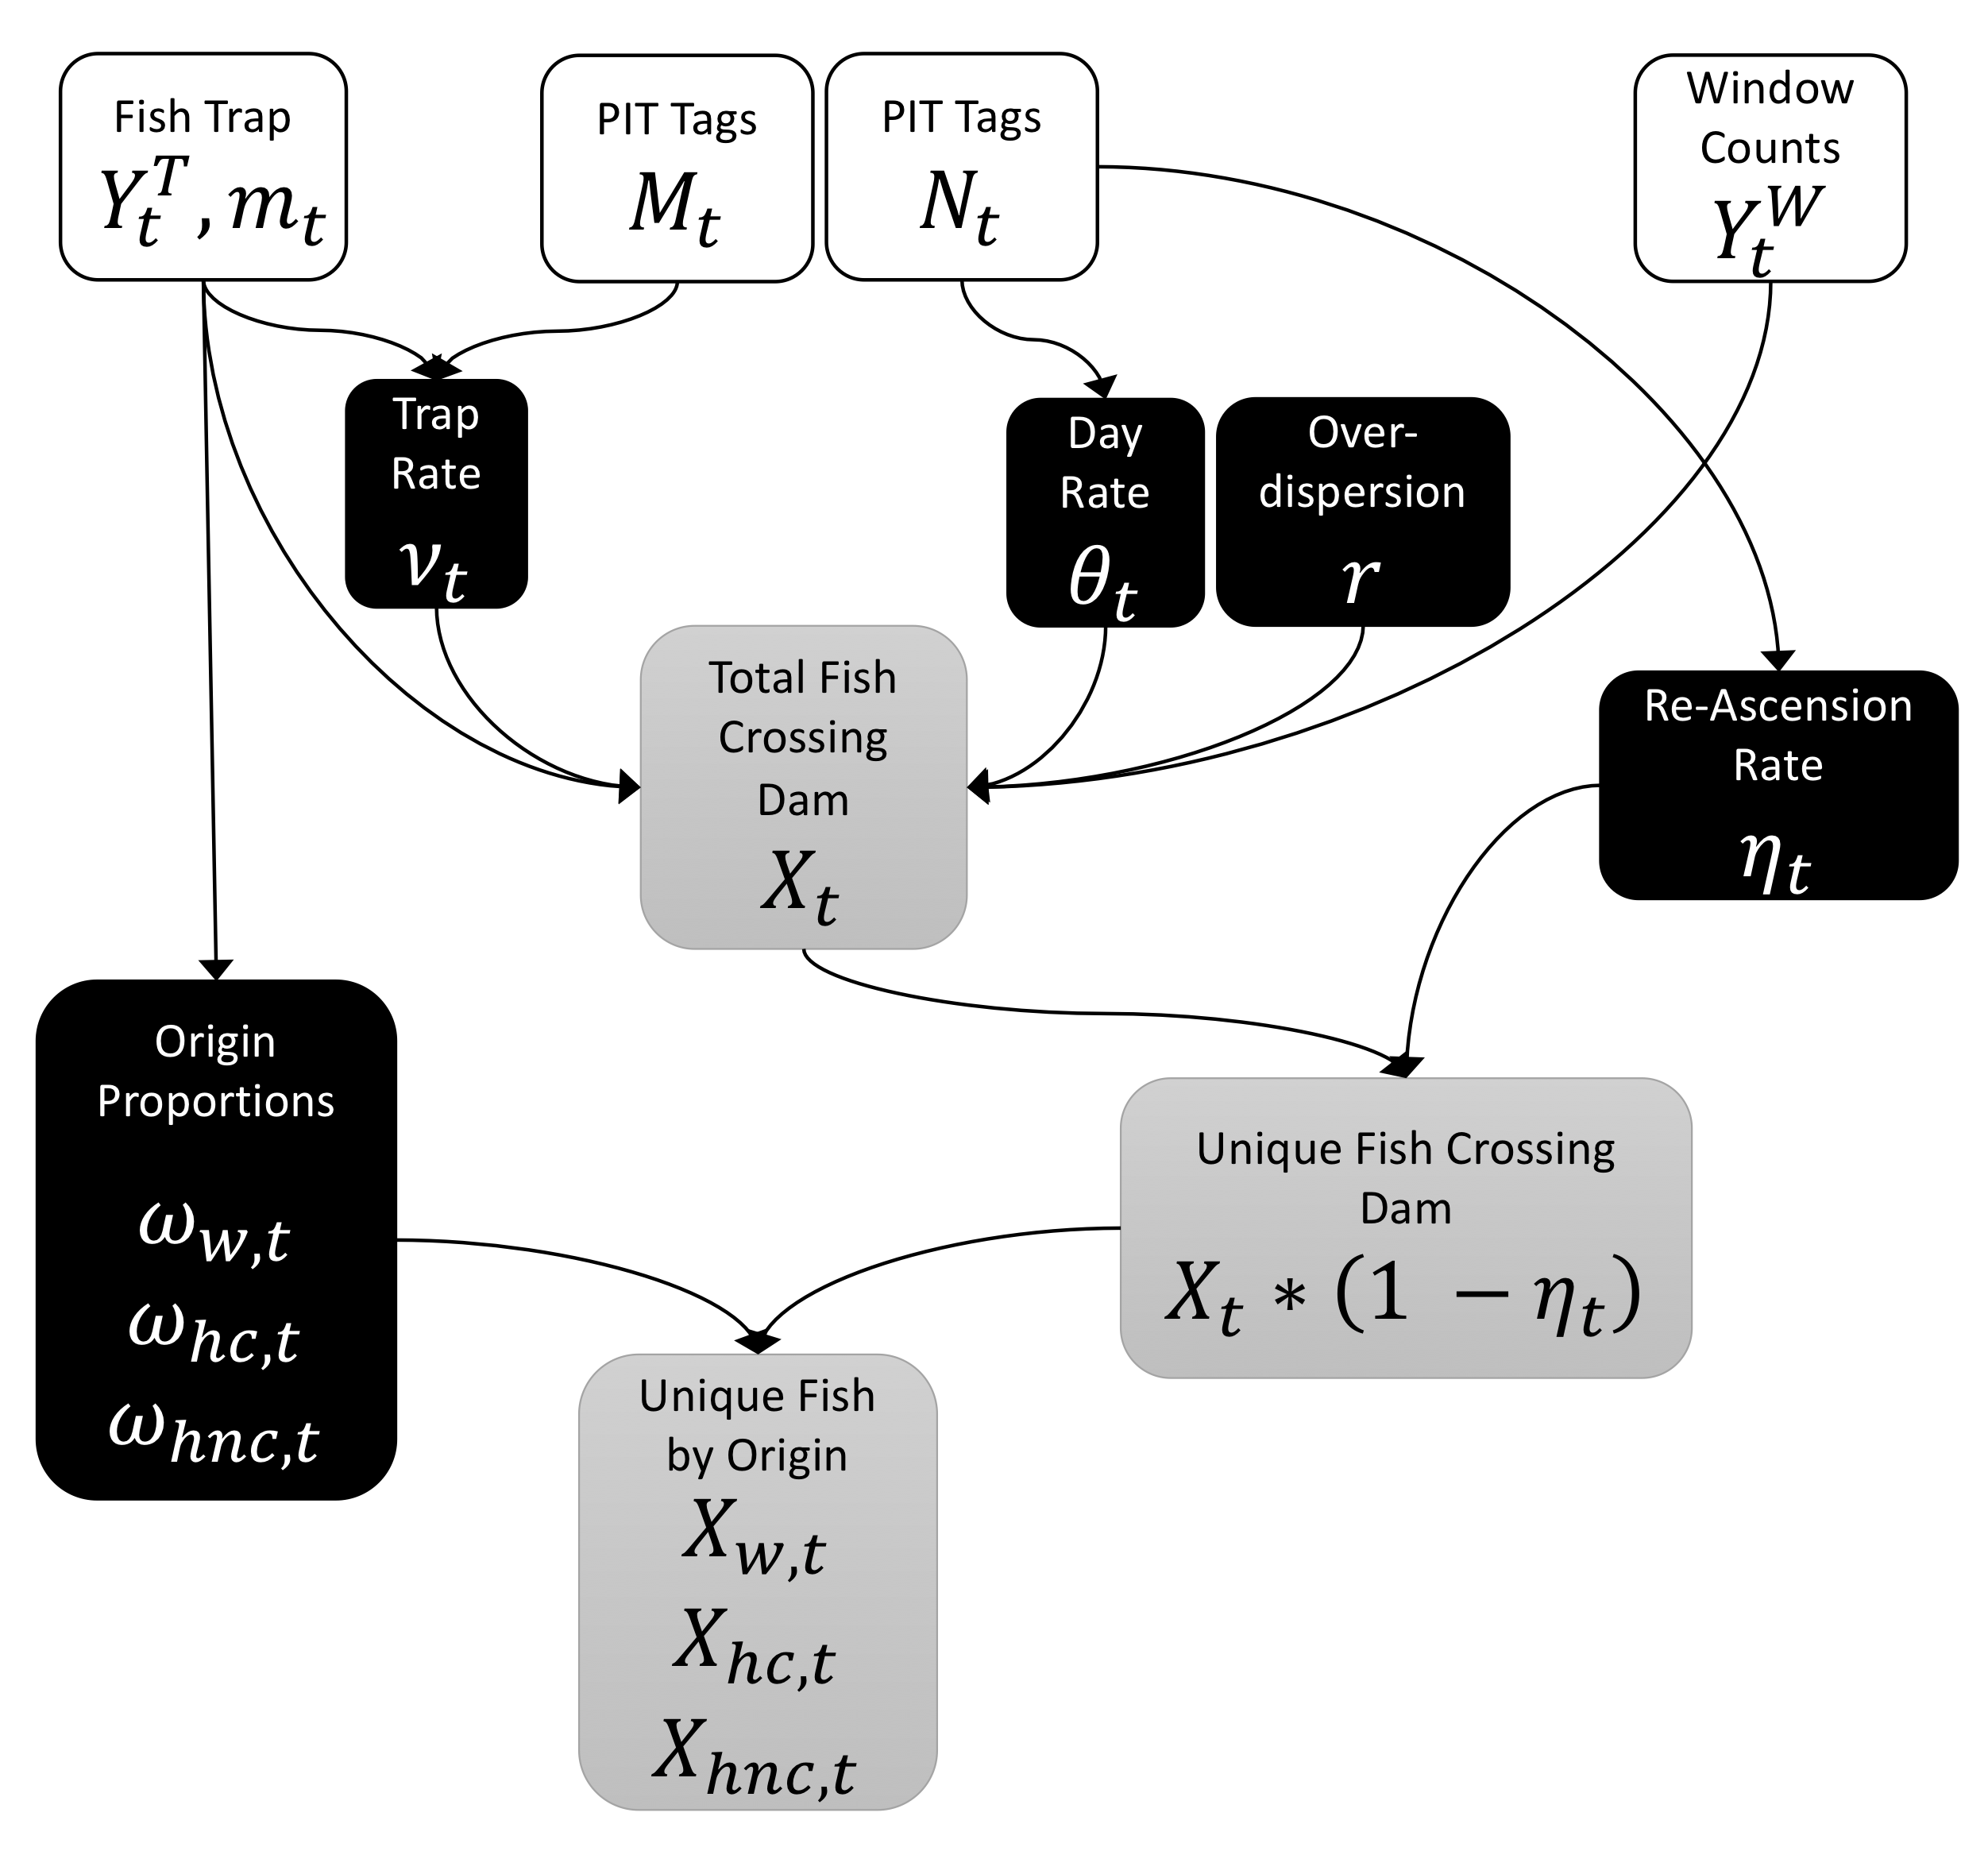
\includegraphics[width=1\linewidth]{../figures/ModelSchematic} \caption{Directed acyclic graph showing the STADEM model framework.}\label{fig:dag-fig}
\end{figure}

\newpage

\begin{figure}
\centering
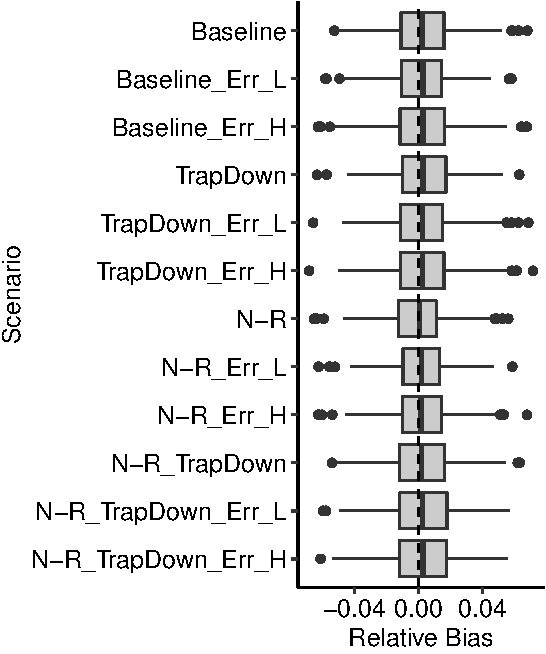
\includegraphics{../figures/rel-bias-lgd-1.pdf}
\caption{\label{fig:rel-bias-lgd}Boxplots of the relative bias of window counts and STADEM estimates for total unique fish and STADEM estimates of unique wild fish across various scenarios (See Table 1).}
\end{figure}

\newpage

\begin{figure}
\centering
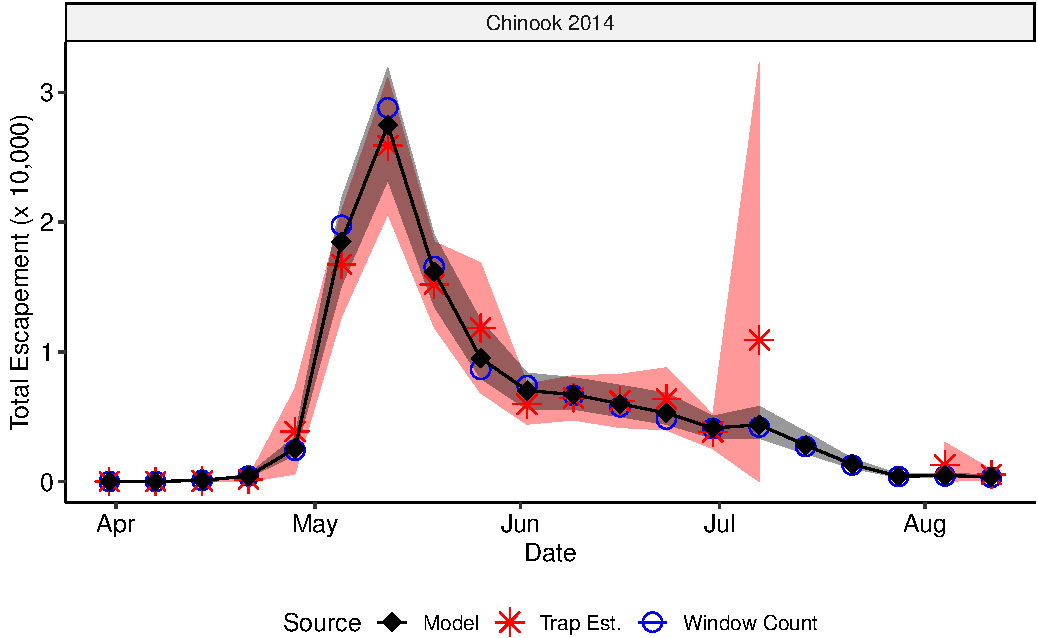
\includegraphics{../figures/jags-fit-fig-1.pdf}
\caption{\label{fig:jags-fit-fig}Time-series plot showing estimates of escapement for spring/summer-run Chinook Salmon in 2014, including window counts, trap estimates and STADEM estimates of unique fish. The dark gray ribbon represents the 95\% credible intervals for STADEM estimates, while the light gray ribbon represents the 95\% confidence intervals for the trap estimates.}
\end{figure}

\newpage

\begin{figure}
\centering
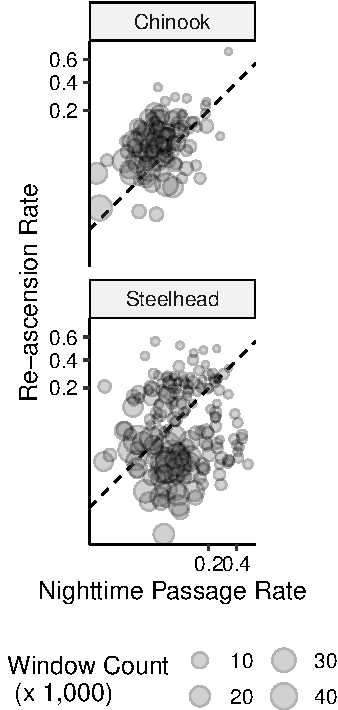
\includegraphics{../figures/night-reasc-diff-fig-1.pdf}
\caption{\label{fig:night-reasc-diff-fig}Nighttime passage rate plotted against re-ascension rate on the logit scale, calculated from observed PIT tags for each week of spawn years 2010-2019. The size of each point is proportional to the window count that week. Points falling below the 1-1 dashed line indicate weekly periods of higher nighttime passage as compared to re-ascension, conversly, points falling above indicate a lower nighttime passage than re-ascension rate.}
\end{figure}

\newpage

\hypertarget{append1}{%
\section{Appendix A - Simulation Details}\label{append1}}

To simulate fish passing a dam, we developed an \(\mathbb{R}\) software function (R Core Team 2020). The function randomly samples observations from assumed probability distribution functions (pdf) with known parameters. Total unique fish, \(N\), and a vector, \(\omega\), containing the proportions of wild (\(w\)), hatchery (\(h\)) and hatchery no-clip (\(hnc\)) fish passing the dam is set to establish known ``truths'' of escapement by origin.

\[
\begin{aligned}
\left[N_{w}, N_{h}, N_{hnc} \right] &= N * \left[\omega_{w}, \omega_{h}, \omega_{hnc} \right]
\end{aligned}
\]

Escapement of each origin is then randomly divided across a set number of populations, \(n\), by randomly drawing proportions, \(\phi_{j,p}\), of origin group \(j\) in each population \(p\) using a Dirichlet pdf. The Dirichlet function is parameterized from a vector, \(\zeta_j\), containing 1's and 0's designating populations with origin \(j\) fish returning. For each population \(p\), \(\zeta_{j,p}\) is drawn from a Bernoulli pdf using the proportion of populations that contain each origin, \(\tau_j\). Wild fish are assumed to be in all populations; \(\tau_w = 1.0\). The product of sampled population proportions \(\phi_{j,p}\) and fixed \(N_j\) yields a random variable of abundance for each origin in each population, \(N_{j,p}\). Summing across origin abundances then gives a random total population abundance, \(N_p\), crossing the dam.

\[
\begin{aligned}
  \zeta_{j,p} &\sim \text{Bernoulli}(\tau_j) \\
  \left[\phi_{j,p=1},  ... , \phi_{j,p=n}\right] &\sim \text{Dir} \left(\zeta_{j,p=1},  ... , \zeta_{j,p=n} \right) \\
  N_{j,p} &= N_j * \phi_{j,p} \\
  N_p &= \sum_{j \in w, h, hnc} N_{j,p}
\end{aligned}
\]

Mean arrival date, \(\bar{a}_p\), for each population returning to the dam is drawn from a normal pdf with hyper-parameters \(\mu_a\) and \(\sigma^2_a\). Similarly, the variance or spread in run-timing within populations is the absolute value of random variables drawn from a normal pdf with hyper-parameters \(\mu_s\) and \(\sigma^2_s\).

\[
\begin{aligned}
 \left[\bar{a}_p, ..., \bar{a}_n\right] &\sim \mathcal{N}(\mu_a, \sigma^2_a) \\
 \left[s_p, ..., s_n\right] &\sim \left | \mathcal{N}(\mu_s, \sigma^2_s) \right |
\end{aligned}
\]

After sampling the mean date of arrival and variances for each population, the date of arrival, \(a_{i,p}\), for individual fish, \(i\), within each population are drawn from a normal pdf with population parameters \(\bar{a}_p\) and \(s^2_p\). This simulates a random arrival day that is similar for all fish returning to the same population, regardless of origin.

\[
\begin{aligned}
 date_{i,p} &\sim \mathcal{N}(\bar{a}_p, s^2_p) \\
\end{aligned}
\]

To model different fish behavior and dam operational scenarios, seven additional attributes are randomly assigned to each individual fish. Each attribute is randomly assigned a TRUE/FALSE using a Bernoulli pdf and a fixed probability parameter. Fish passage during the day-time (i.e., during periods of window operation) is modeled using one minus the night-time passage rate (\(1 - \nu\)). Window observations are conditioned on fish passing during the day and being observed at a set rate, \(\gamma\). Whether fish \(i\) is sampled by the adult trap is modeled on the weekly set trap rate, \(\delta_t\). The rate of previously PIT-tagged fish is determined by \(\lambda\), and their subsequent detection at the ladder PIT antenna is governed by \(\kappa\). Fallback behavior is modeled with a common rate across all populations, \(\psi\). Re-ascension occurs with probability \(\rho\), conditioned on fish \(i\) falling back. If fish \(i\) falls back and re-ascends, the entire process described above is repeated, with some time-lag between initial ascension and re-ascension that is governed by a Poisson pdf with mean = 2 days. Fish may fallback and re-ascend up to 3 times, allowing for the possibility of the same fish being counted or trapped multiple times.

\[
\begin{aligned}
  day_{i} &\sim \text{Bern}(1-\nu) \\
  window_{i} &\sim \text{Bern}(\gamma \times day_i) \\
  trapped_{i} &\sim \text{Bern}(\delta_t) \\
  tagged_{i} &\sim \text{Bern}(\lambda) \\
  ladder_{i} &\sim \text{Bern}(\kappa \times tagged_i) \\  
  fallback_{i} &\sim \text{Bern}(\psi) \\
  re-ascend_{i} &\sim \text{Bern}(\rho \times fallback_i)
\end{aligned}
\]

Simulation parameters for model evaluations were set to mimic typical escapement of spring/summer Chinook Salmon to LGD with similar origin proportions, marking rates and run timing as those observed from return years 2010 - 2015. Escapement of each origin (\(N_j\)) was set at 25,000 wild, 70,000 hatchery and 5,000 hatchery no-clips spread randomly across 25 populations (\(n\)). Of the 25 populations, each had a 1.0 probability of containing wild fish, 0.50 probability of having hatchery fish and 0.15 probability of receiving hatchery no-clip (\(\tau_j\)); resulting in an expected 25 wild, 12.5 hatchery and 3.75 hatchery no-clip populations. Mean arrival dates and variability were estimated from PIT-tag detection data queried from the Columbia Basin Research Data Access in Real Time (\href{http://www.cbr.washington.edu/dart/query/pit_adult_window}{DART}) website and organized by release subbasin. Mean arrival date across all subbasins and 2010 - 2015 return years was June \(19^{th}\) (\(\mu_a = 171\)) with a standard deviation of 13 days (\(\sigma_a\)). While the observed spread (i.e., variance) of arrival dates within subbasins was determined to have a mean (\(\mu_s\)) of 22 days and a standard deviation of 7 days (\(\sigma_s\)).

For the specific simulated scenarios, we were interested in STADEM model estimates of origin specific escapement from the combinations of two separate trapping rates, two fallback, re-ascension and night-passage combinations and three window count error rates; resulting in twelve different scenarios. First, trapping rates were set static at 0.15 across all weeks for six scenarios to mimic an optimum trap operation for an expected return of 25,000 wild fish (i.e., trap \(\approx\) 4,000 wild fish). For the remaining six scenarios, trapping rates for weeks 30, 31 and 32 (i.e., July \(22^{nd}\) to August \(11^{th}\)) were changed to 0.00 to test STADEM sensitivities to potential trap shut downs similar to those observed in 2013, 2014 and 2015 (Ogden 2014, 2016b, 2016a). To simulate and control the number of re-ascending and night-time passing fish to model response, we altered fallback and night-time passage rates while holding the re-ascension rate constant at \(\rho = 1.0\). Altering fallback rates and holding re-ascension constant allowed for a more simple control of the number of fish re-ascending; because the number of re-ascending fish is a function of the number of fallbacks and the re-ascension rate. Six scenarios had equal rates of fallback and night-time passage set at \(\psi = \nu = 0.06\) (Boggs et al. 2004) which means other estimator assumptions (Schrader et al. 2013). The other six scenarios set fallback at \(\psi = 0.10\) and night-time passage at \(\nu = 0.05\) to create a 5.0\% positive bias of unique fish at the window. A potential 5.0\% weekly bias was determined from PIT-tag data and within the range of observed weekly difference for return years 2010 - 2015 (Figure \ref{fig:night-reasc-diff-fig}). Finally, we desired to test the sensitivities of STADEM to potential rates of window count error; 0\%, 5\% and 10\% (Hatch et al. 1994). To simulate window count error, we assumed the observed daily count was a random variable from a normal distribution with a mean equal to the true daily count, and a standard deviation equal to the applied error rate (i.e., 0\%, 5\%, 10\%) multiplied by the true daily count. This method simulated observed counts as unbiased, and allowed for possible under and overcounts at the window.

All code for simulating data and fitting STADEM to that data can be found at \url{https://www.github.com/KevinSee/ManuscriptSTADEM}.

\end{document}
